\chapter*{Приложение Г}
\addcontentsline{toc}{chapter}{Приложение Г}

\begin{figure}[H]
    
\includegraphics[width=1\linewidth]{img/1.png}
    \caption{Презентация -- слайд 1}
\end{figure}
\noindent

\begin{figure}[H]
    
\includegraphics[width=1\linewidth]{img/2.png}
    \caption{Презентация -- слайд 2}
\end{figure}
\noindent

\begin{figure}[H]
    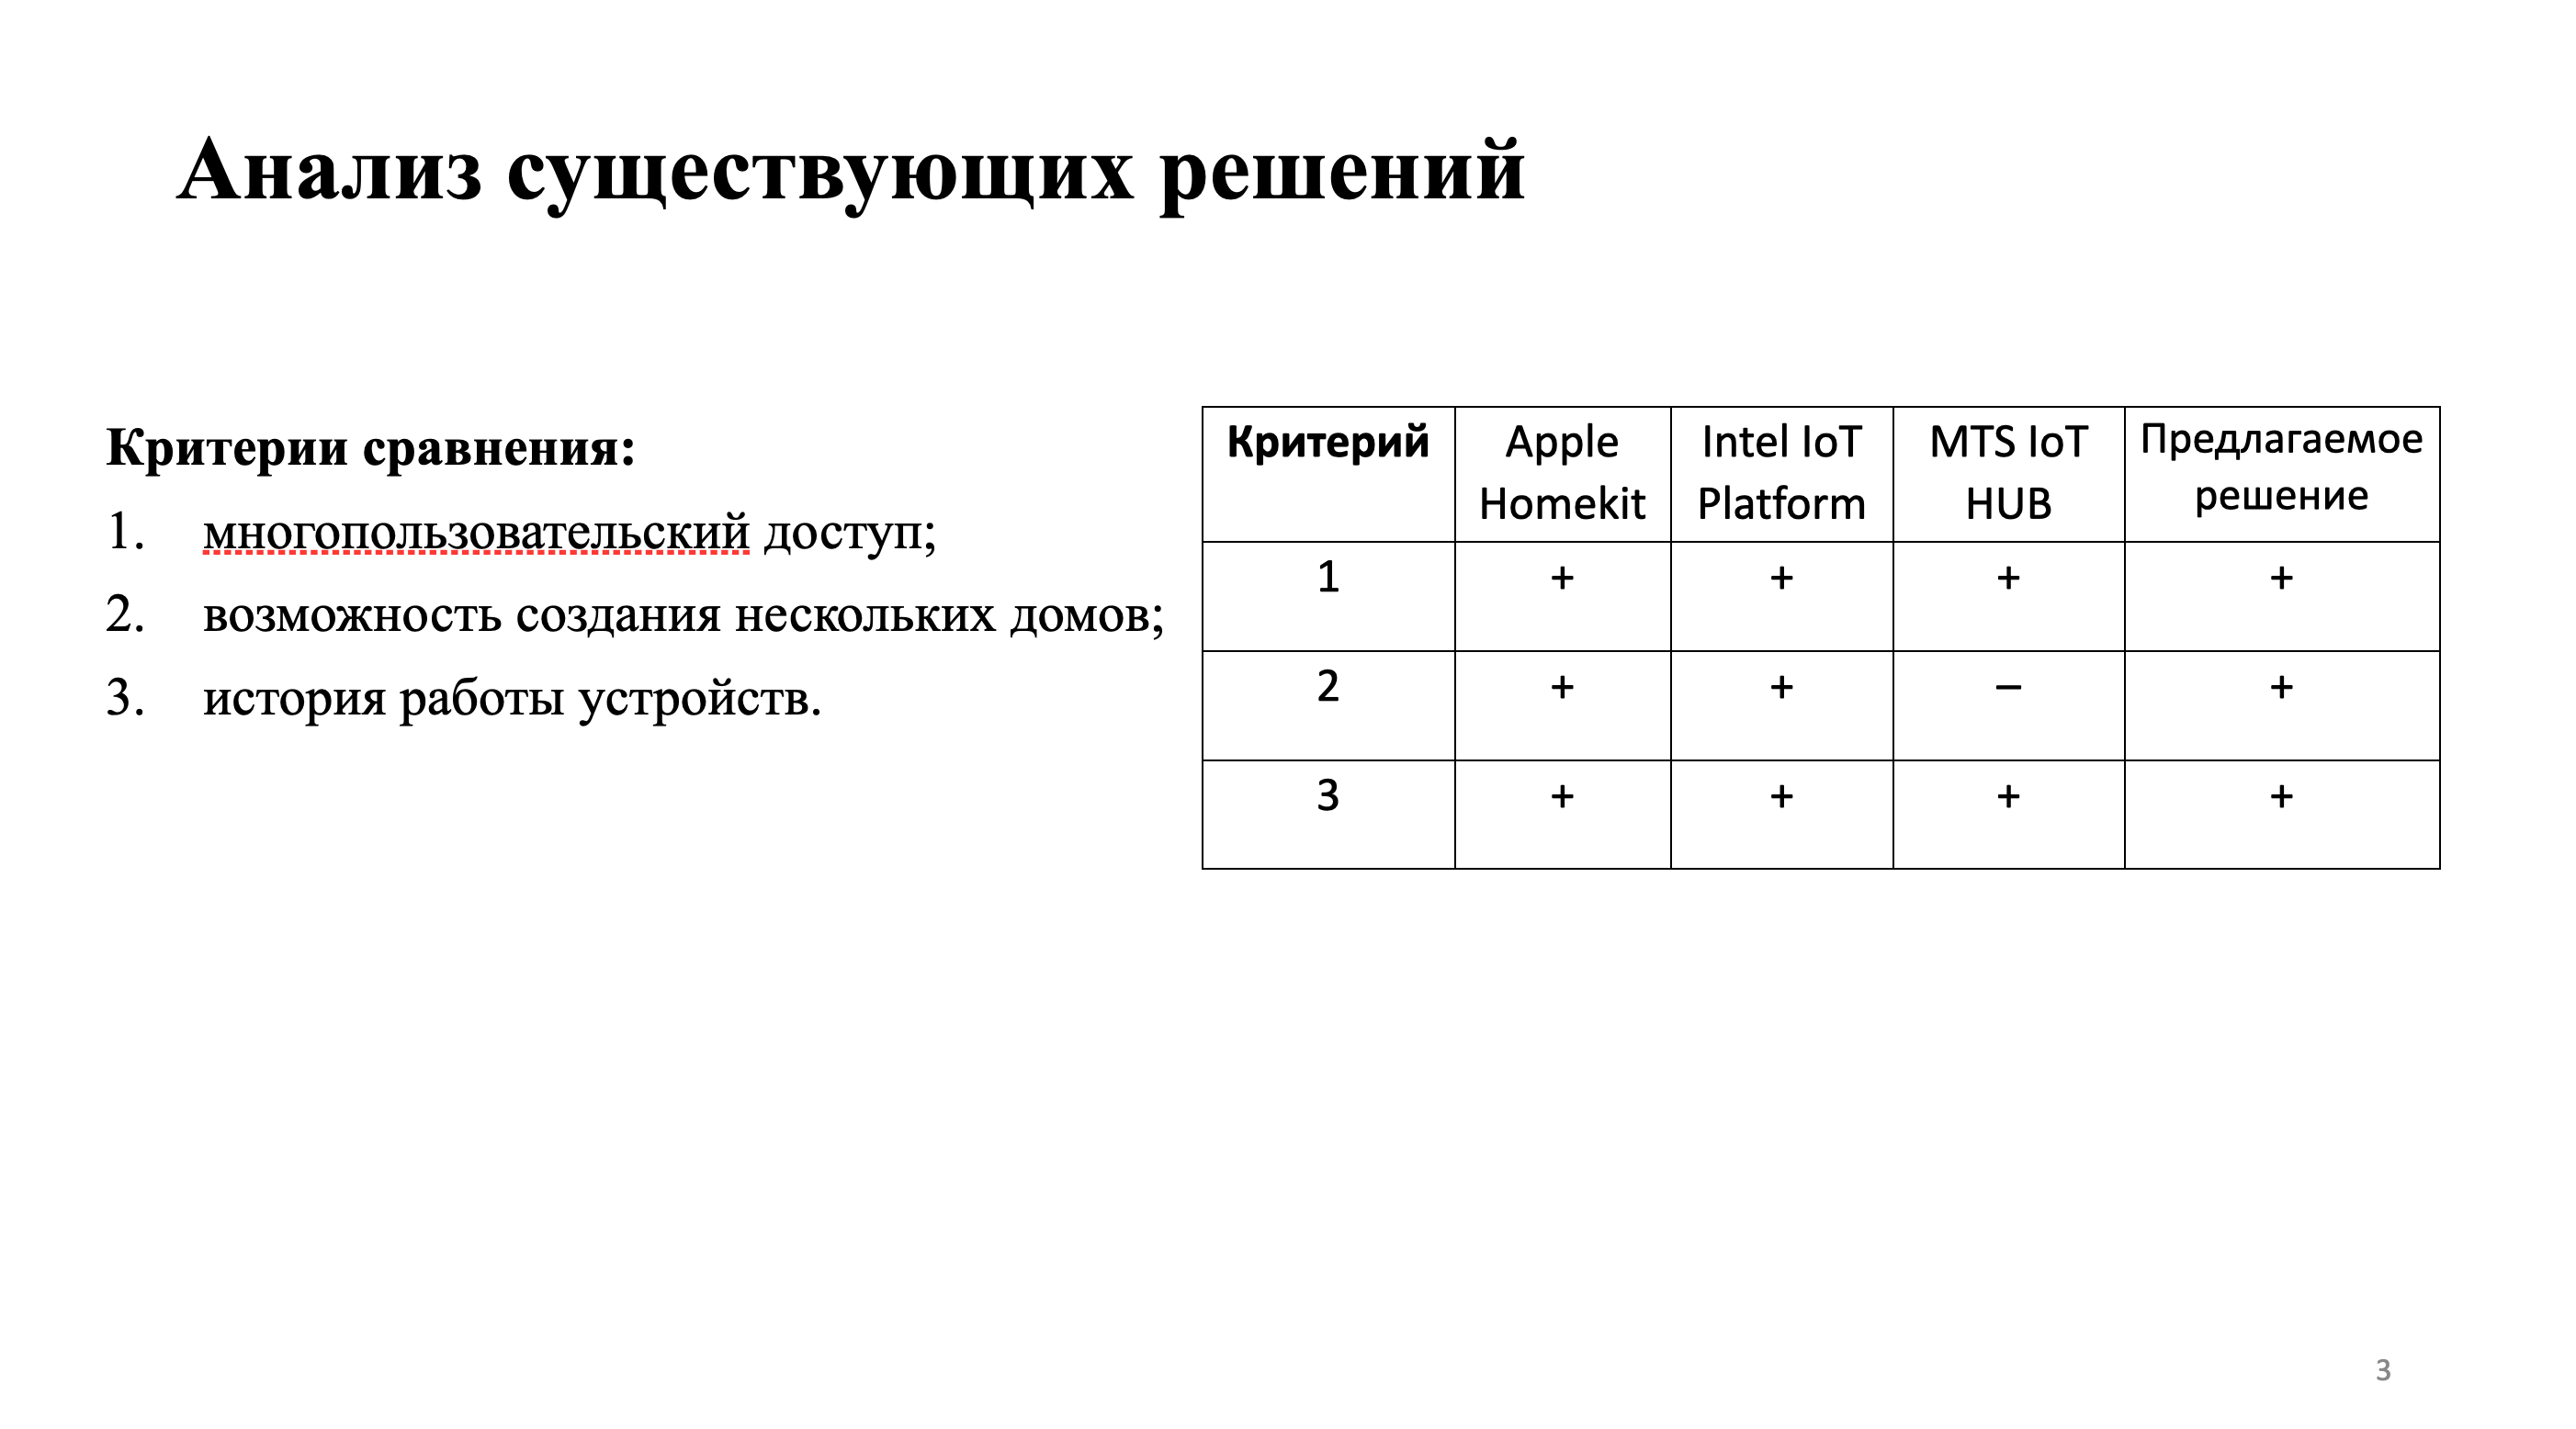
\includegraphics[width=1\linewidth]{img/3.png}
    \caption{Презентация -- слайд 3}
\end{figure}
\noindent

\begin{figure}[H]
    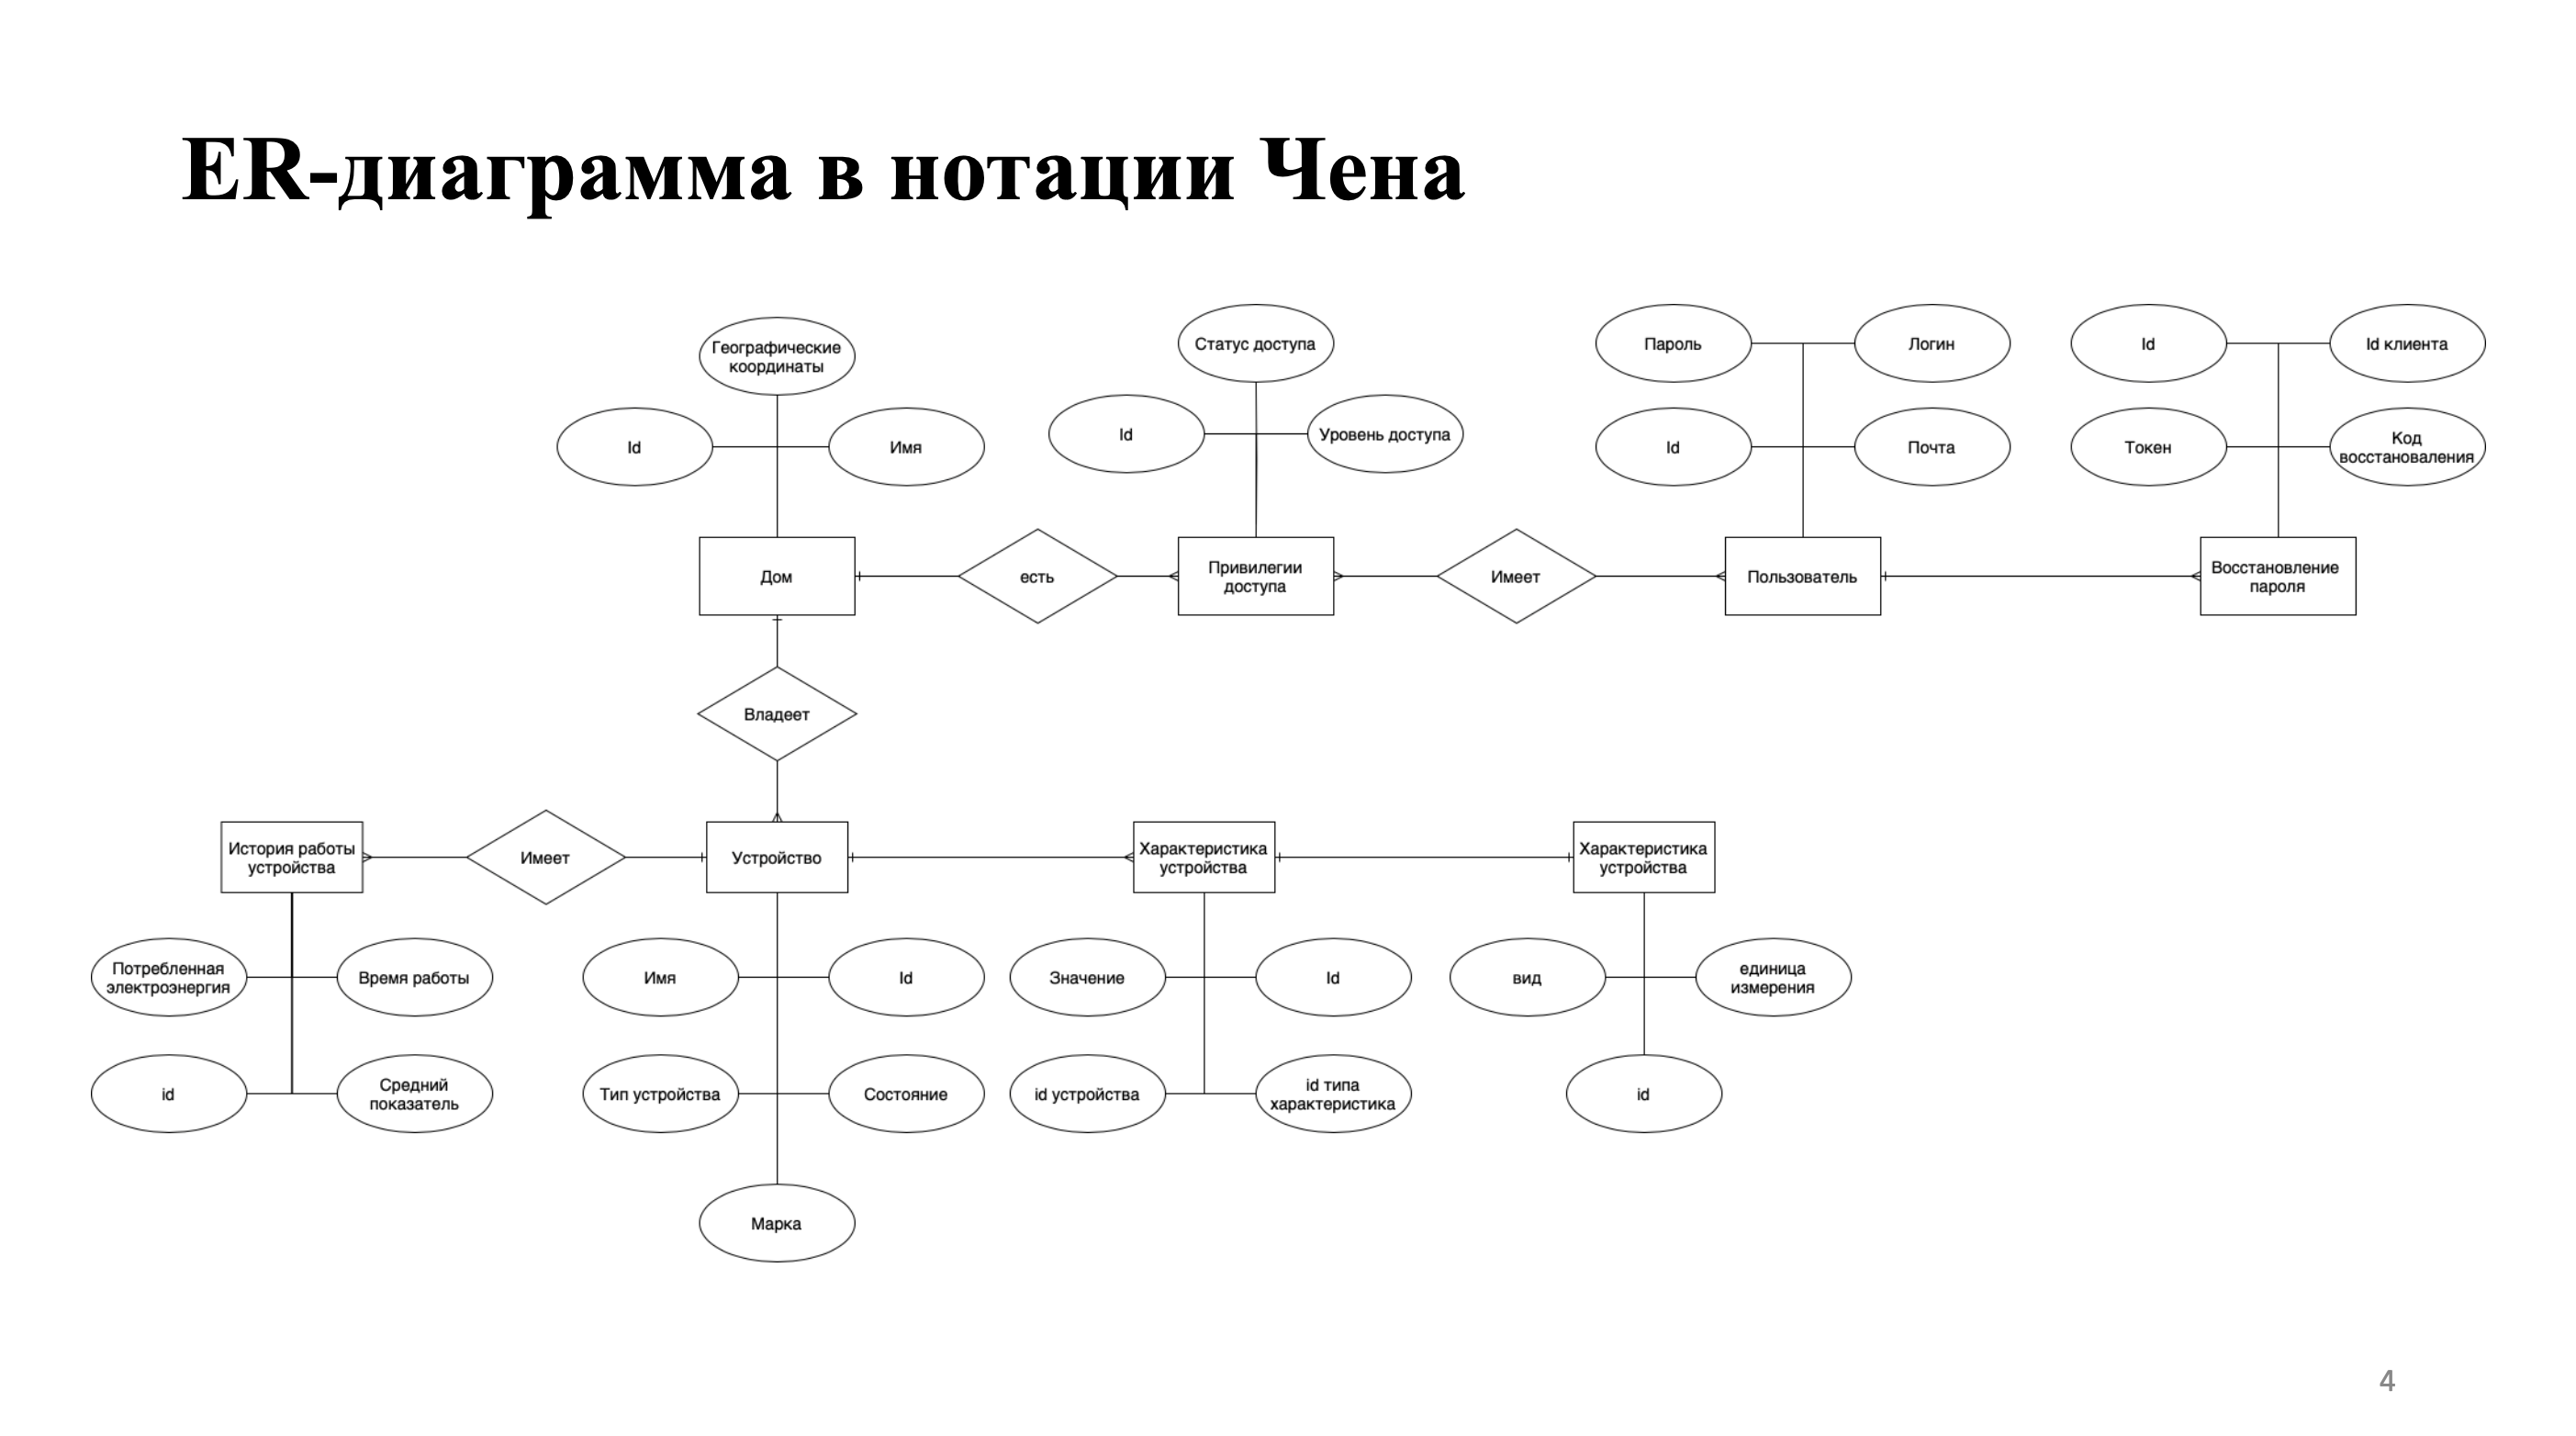
\includegraphics[width=1\linewidth]{img/4.png}
    \caption{Презентация -- слайд 4}
\end{figure}
\noindent

\begin{figure}[H]
    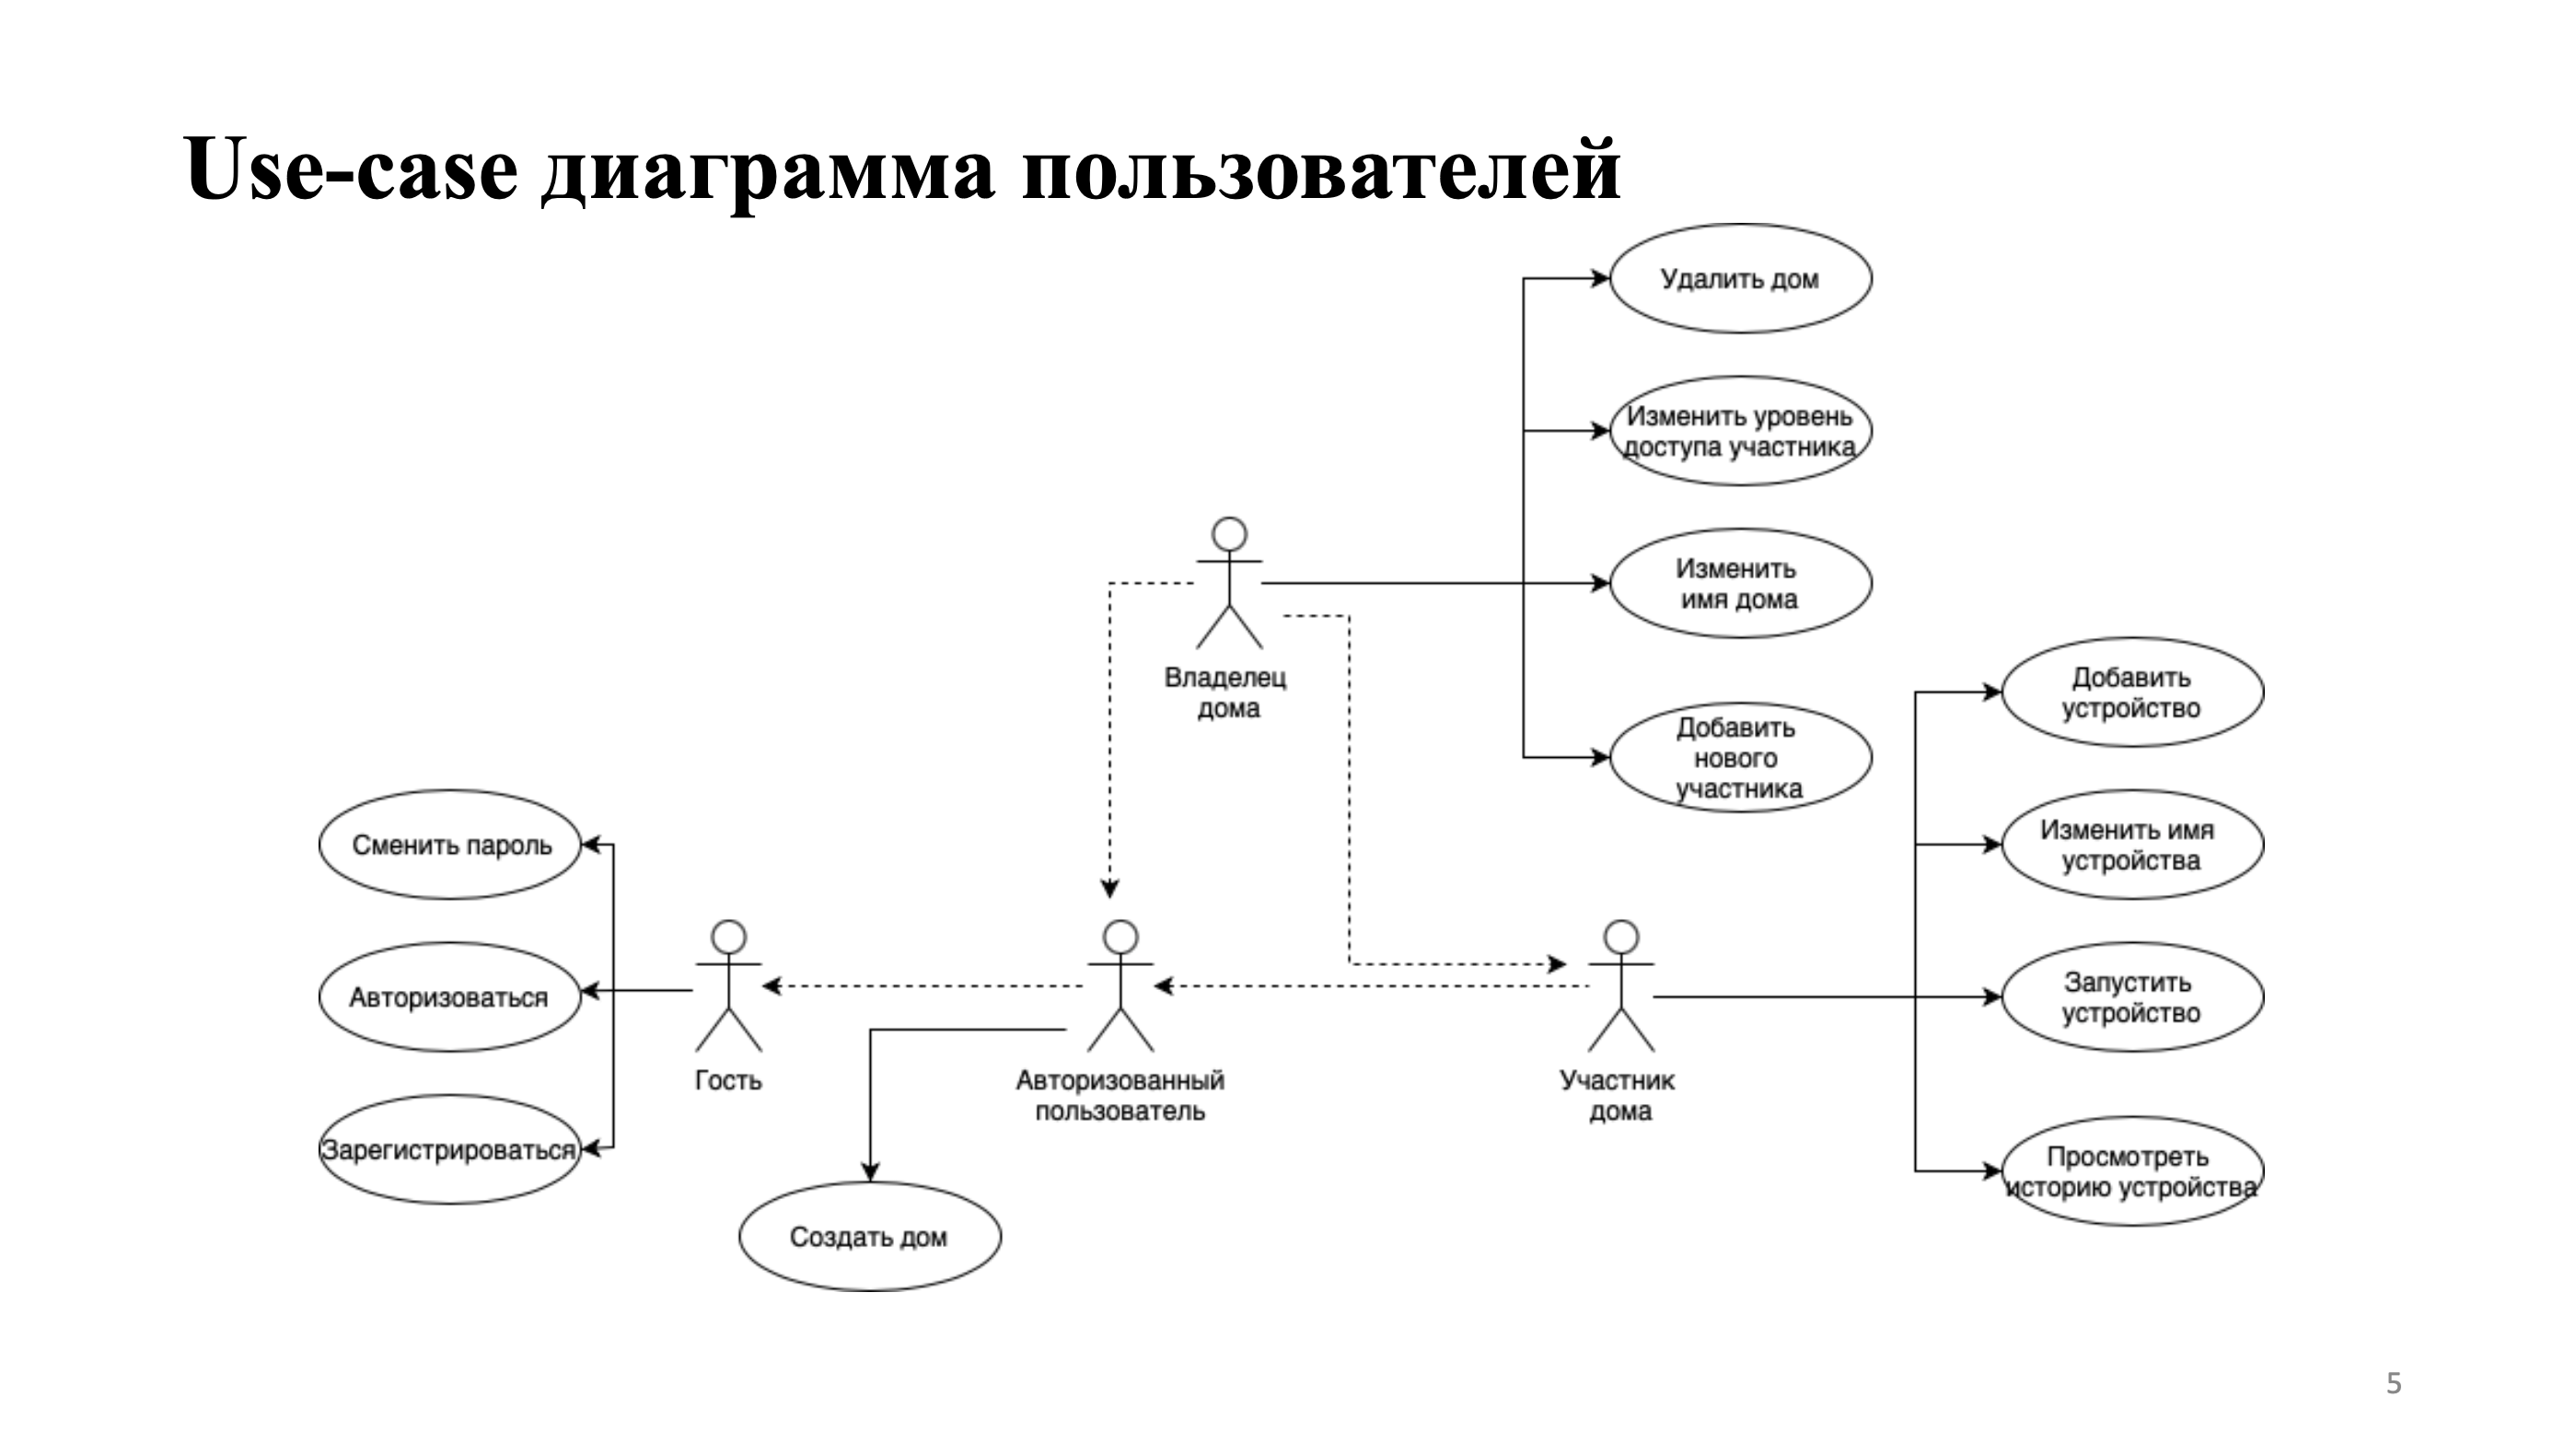
\includegraphics[width=1\linewidth]{img/5.png}
    \caption{Презентация -- слайд 5}
\end{figure}
\noindent

\begin{figure}[H]
    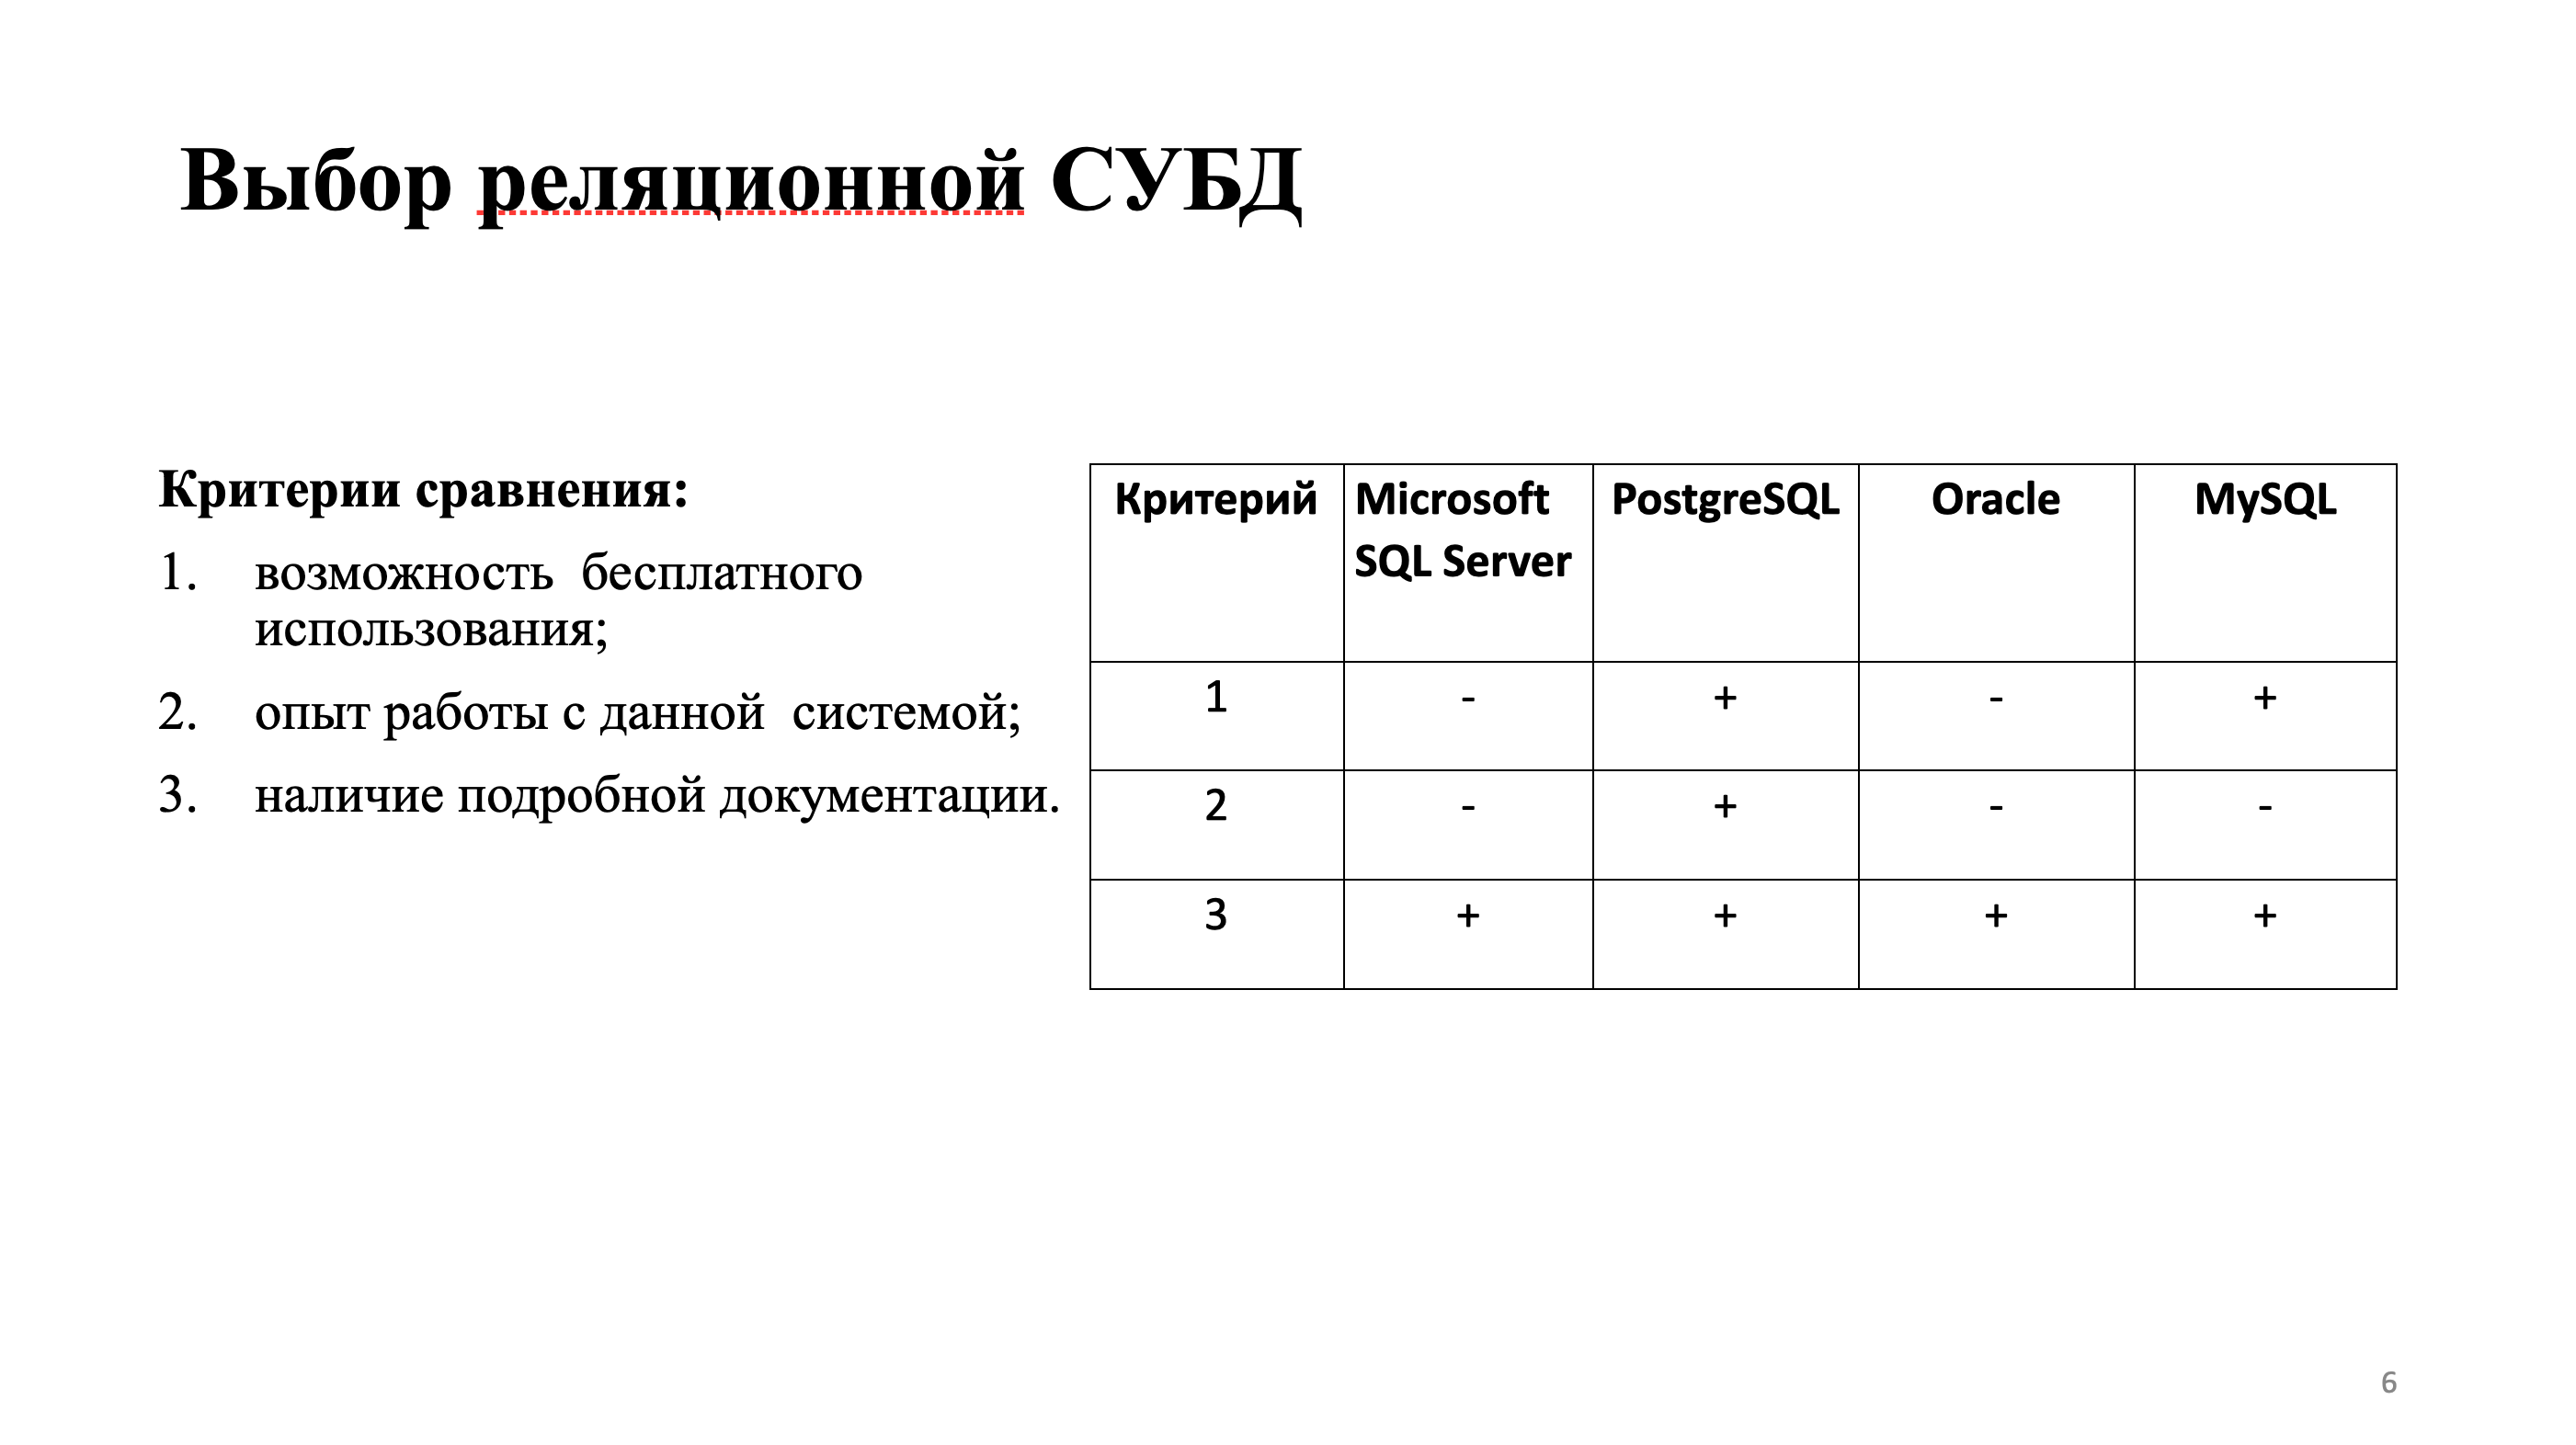
\includegraphics[width=1\linewidth]{img/6.png}
    \caption{Презентация -- слайд 6}
\end{figure}
\noindent

\begin{figure}[H]
    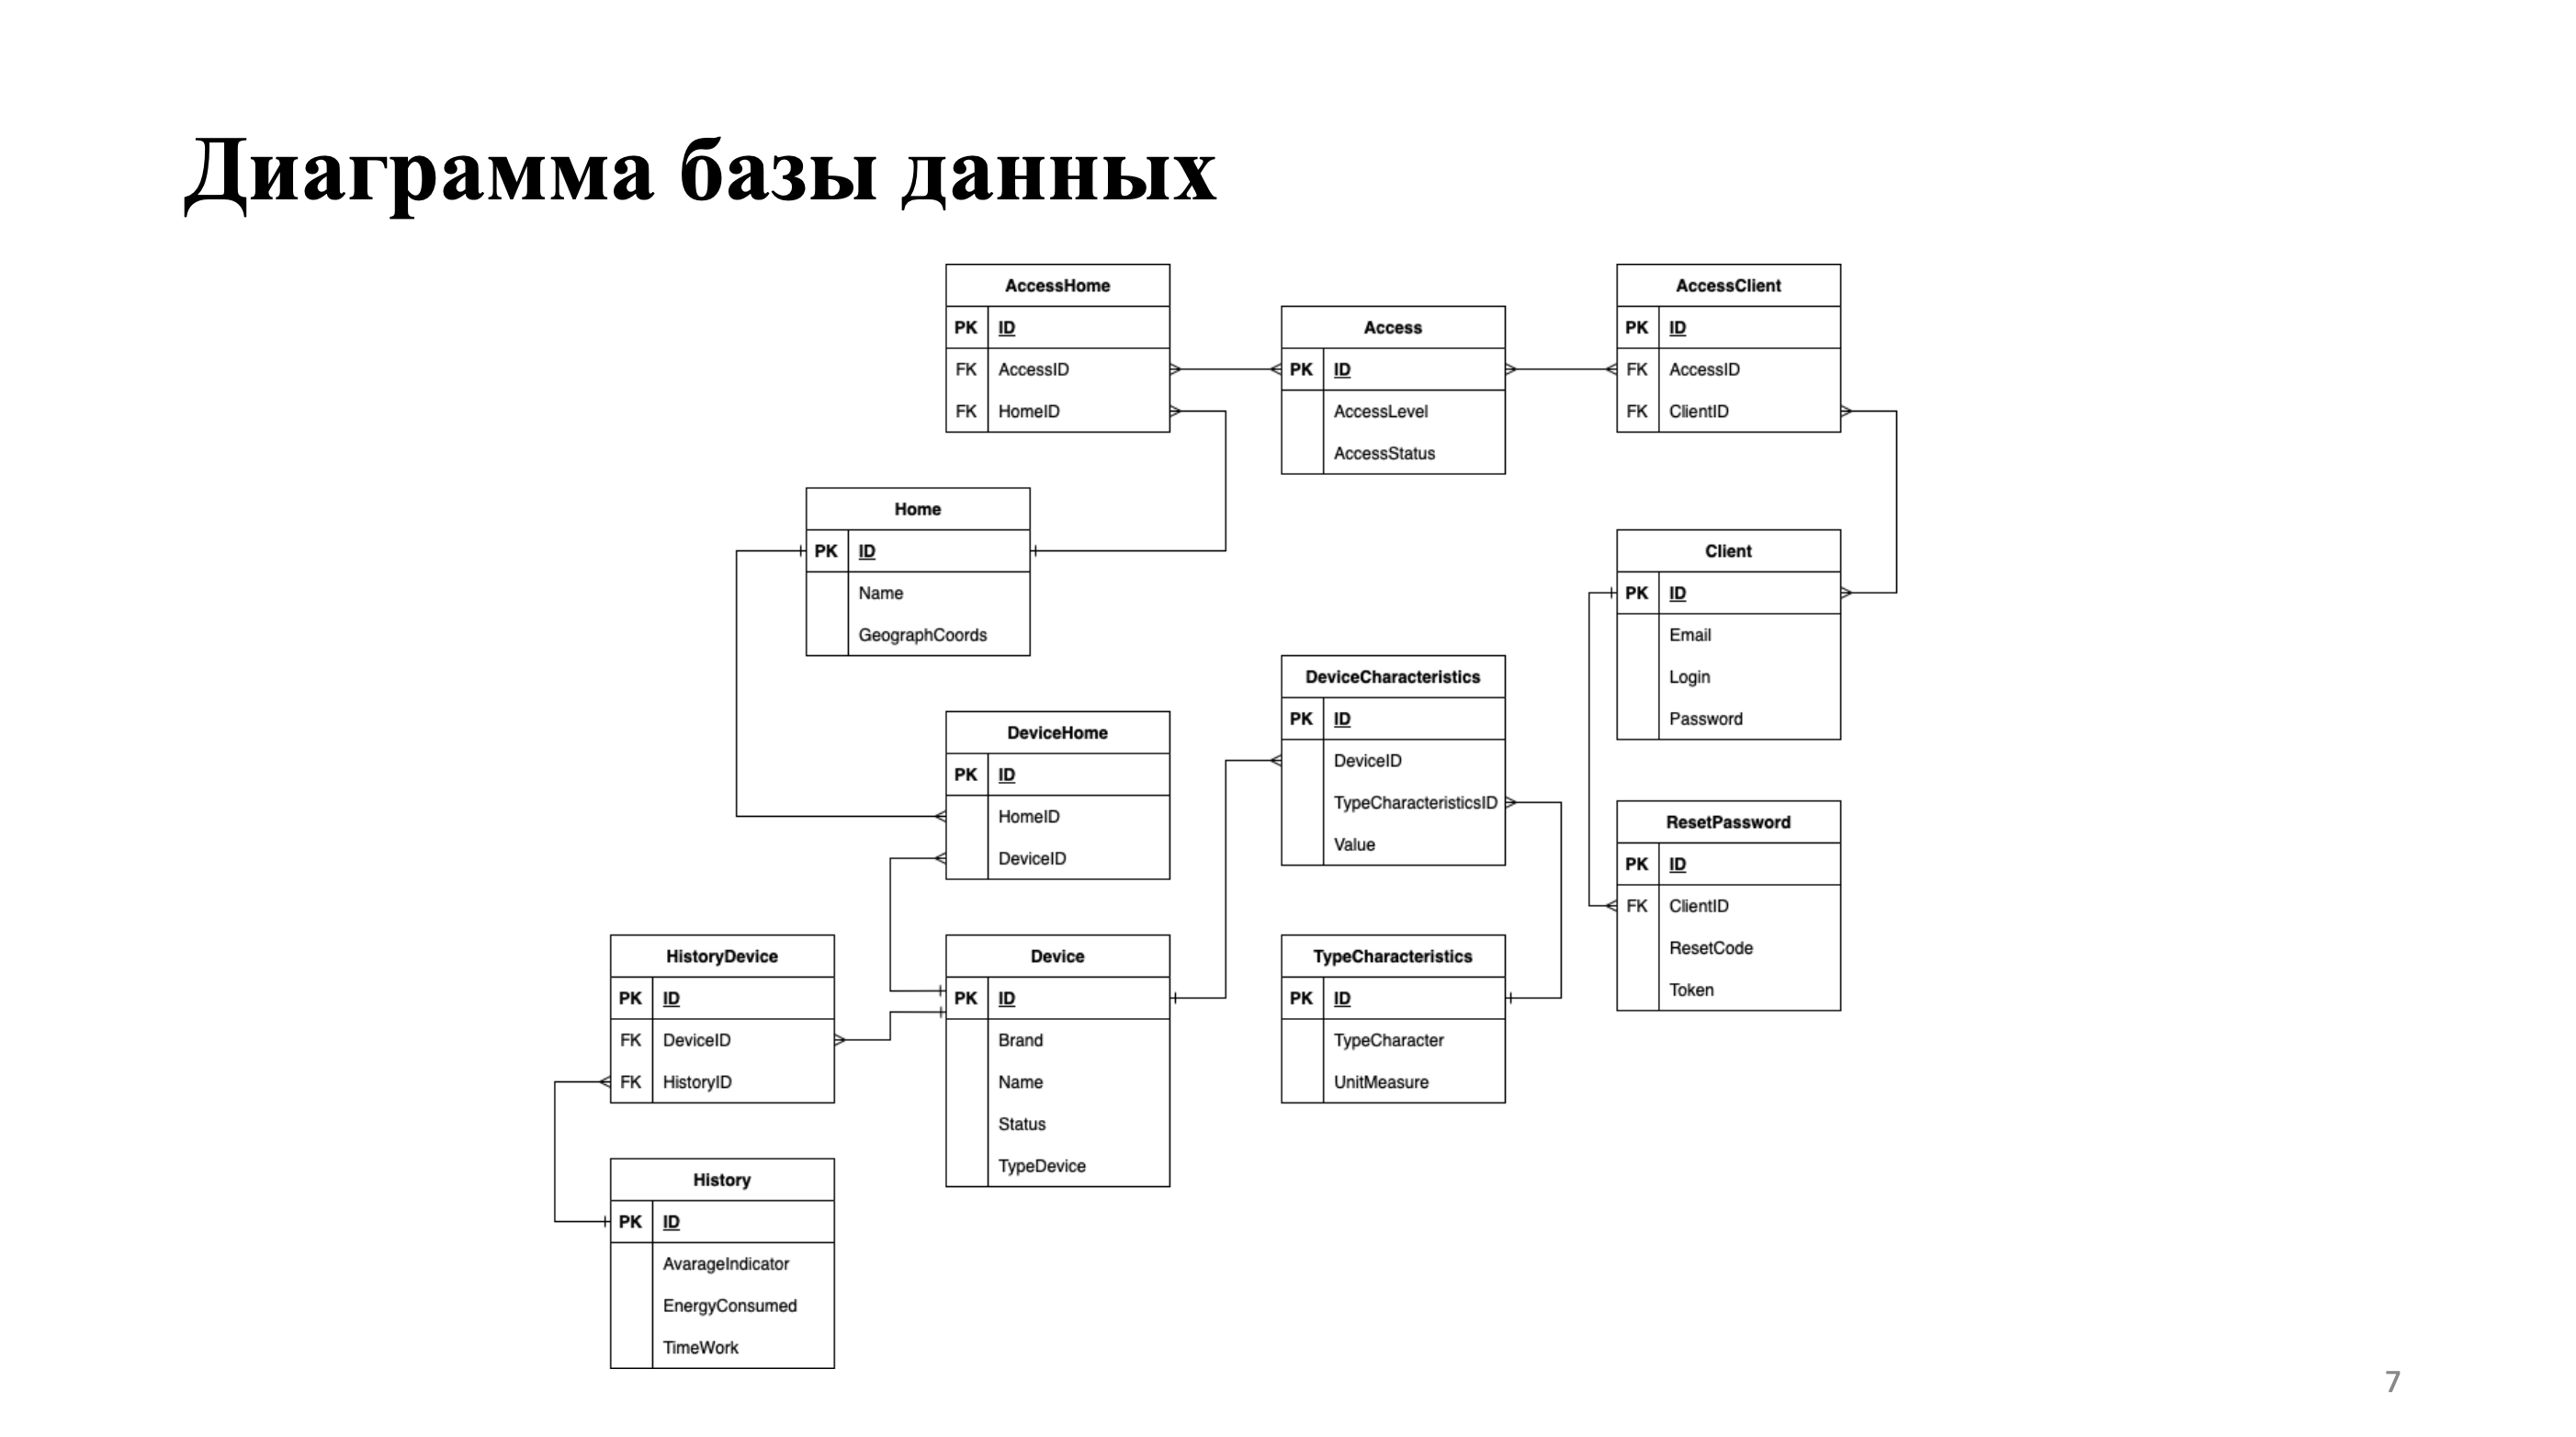
\includegraphics[width=1\linewidth]{img/7.png}
    \caption{Презентация -- слайд 7}
\end{figure}
\noindent

\begin{figure}[H]
    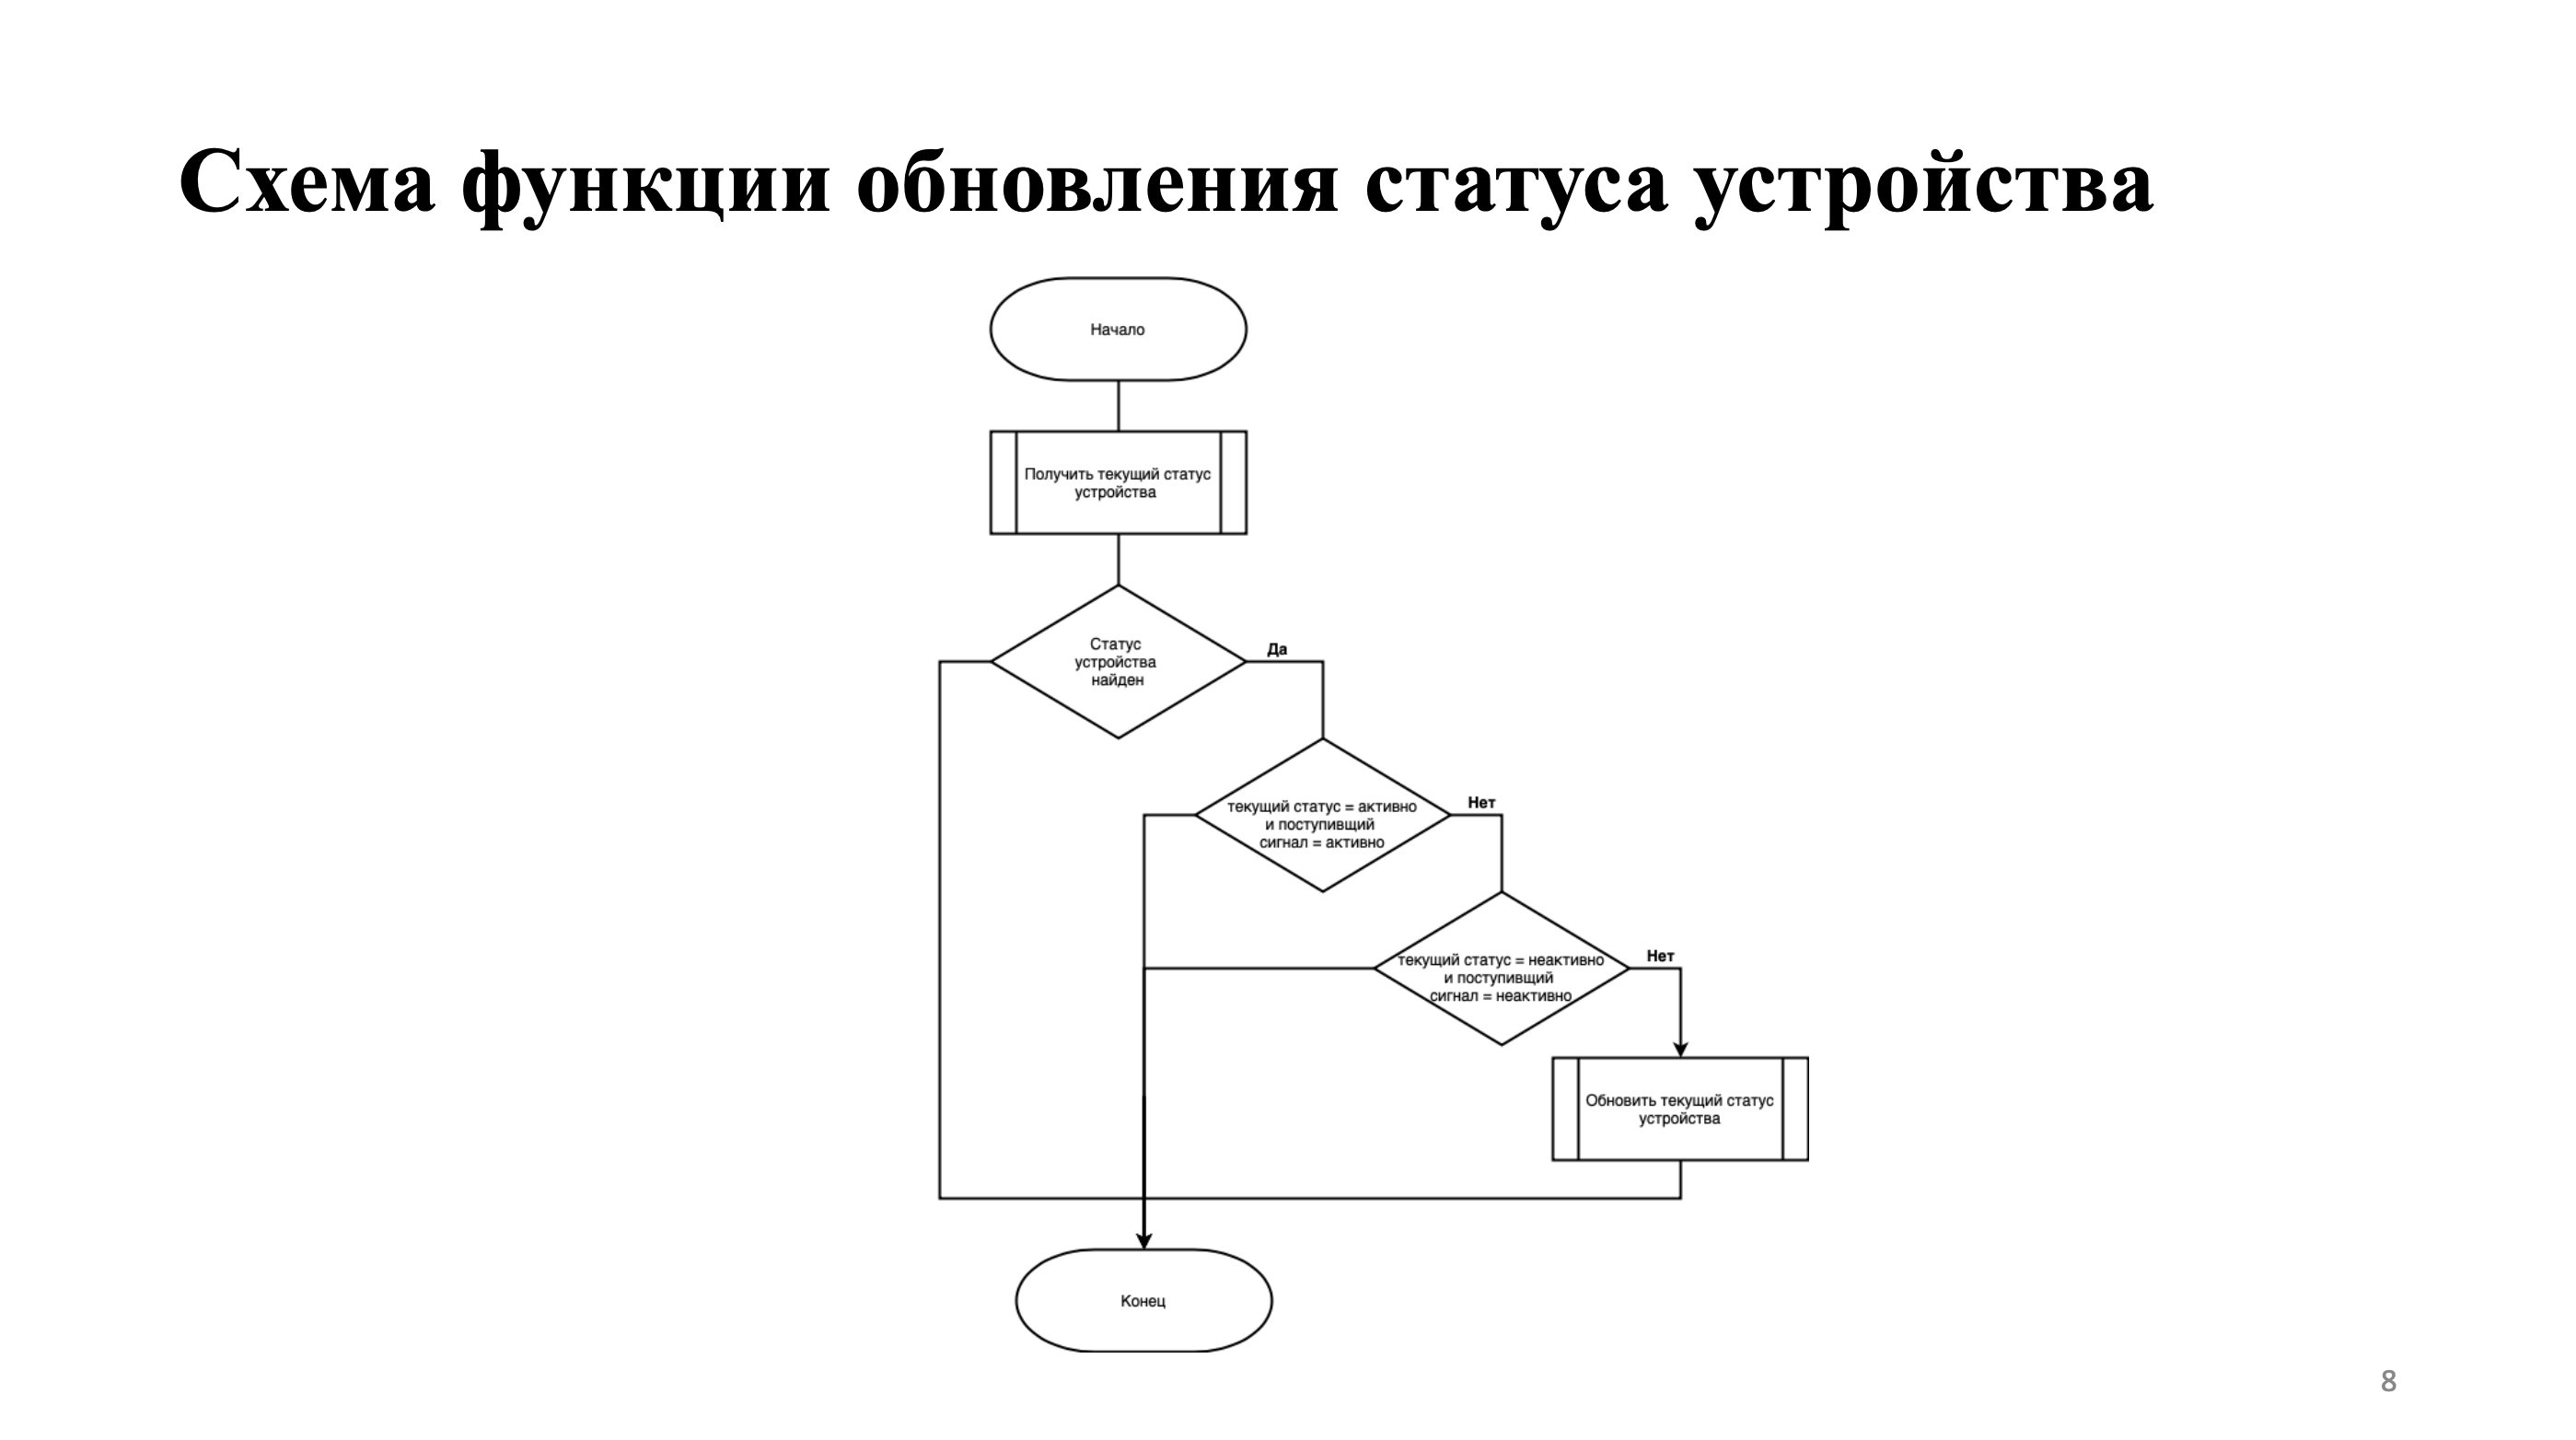
\includegraphics[width=1\linewidth]{img/8.png}
    \caption{Презентация -- слайд 8}
\end{figure}
\noindent

\begin{figure}[H]
    
\includegraphics[width=1\linewidth]{img/9.png}
    \caption{Презентация -- слайд 9}
\end{figure}
\noindent

\begin{figure}[H]
    
\includegraphics[width=1\linewidth]{img/10.png}
    \caption{Презентация -- слайд 10}
\end{figure}
\noindent

\begin{figure}[H]
    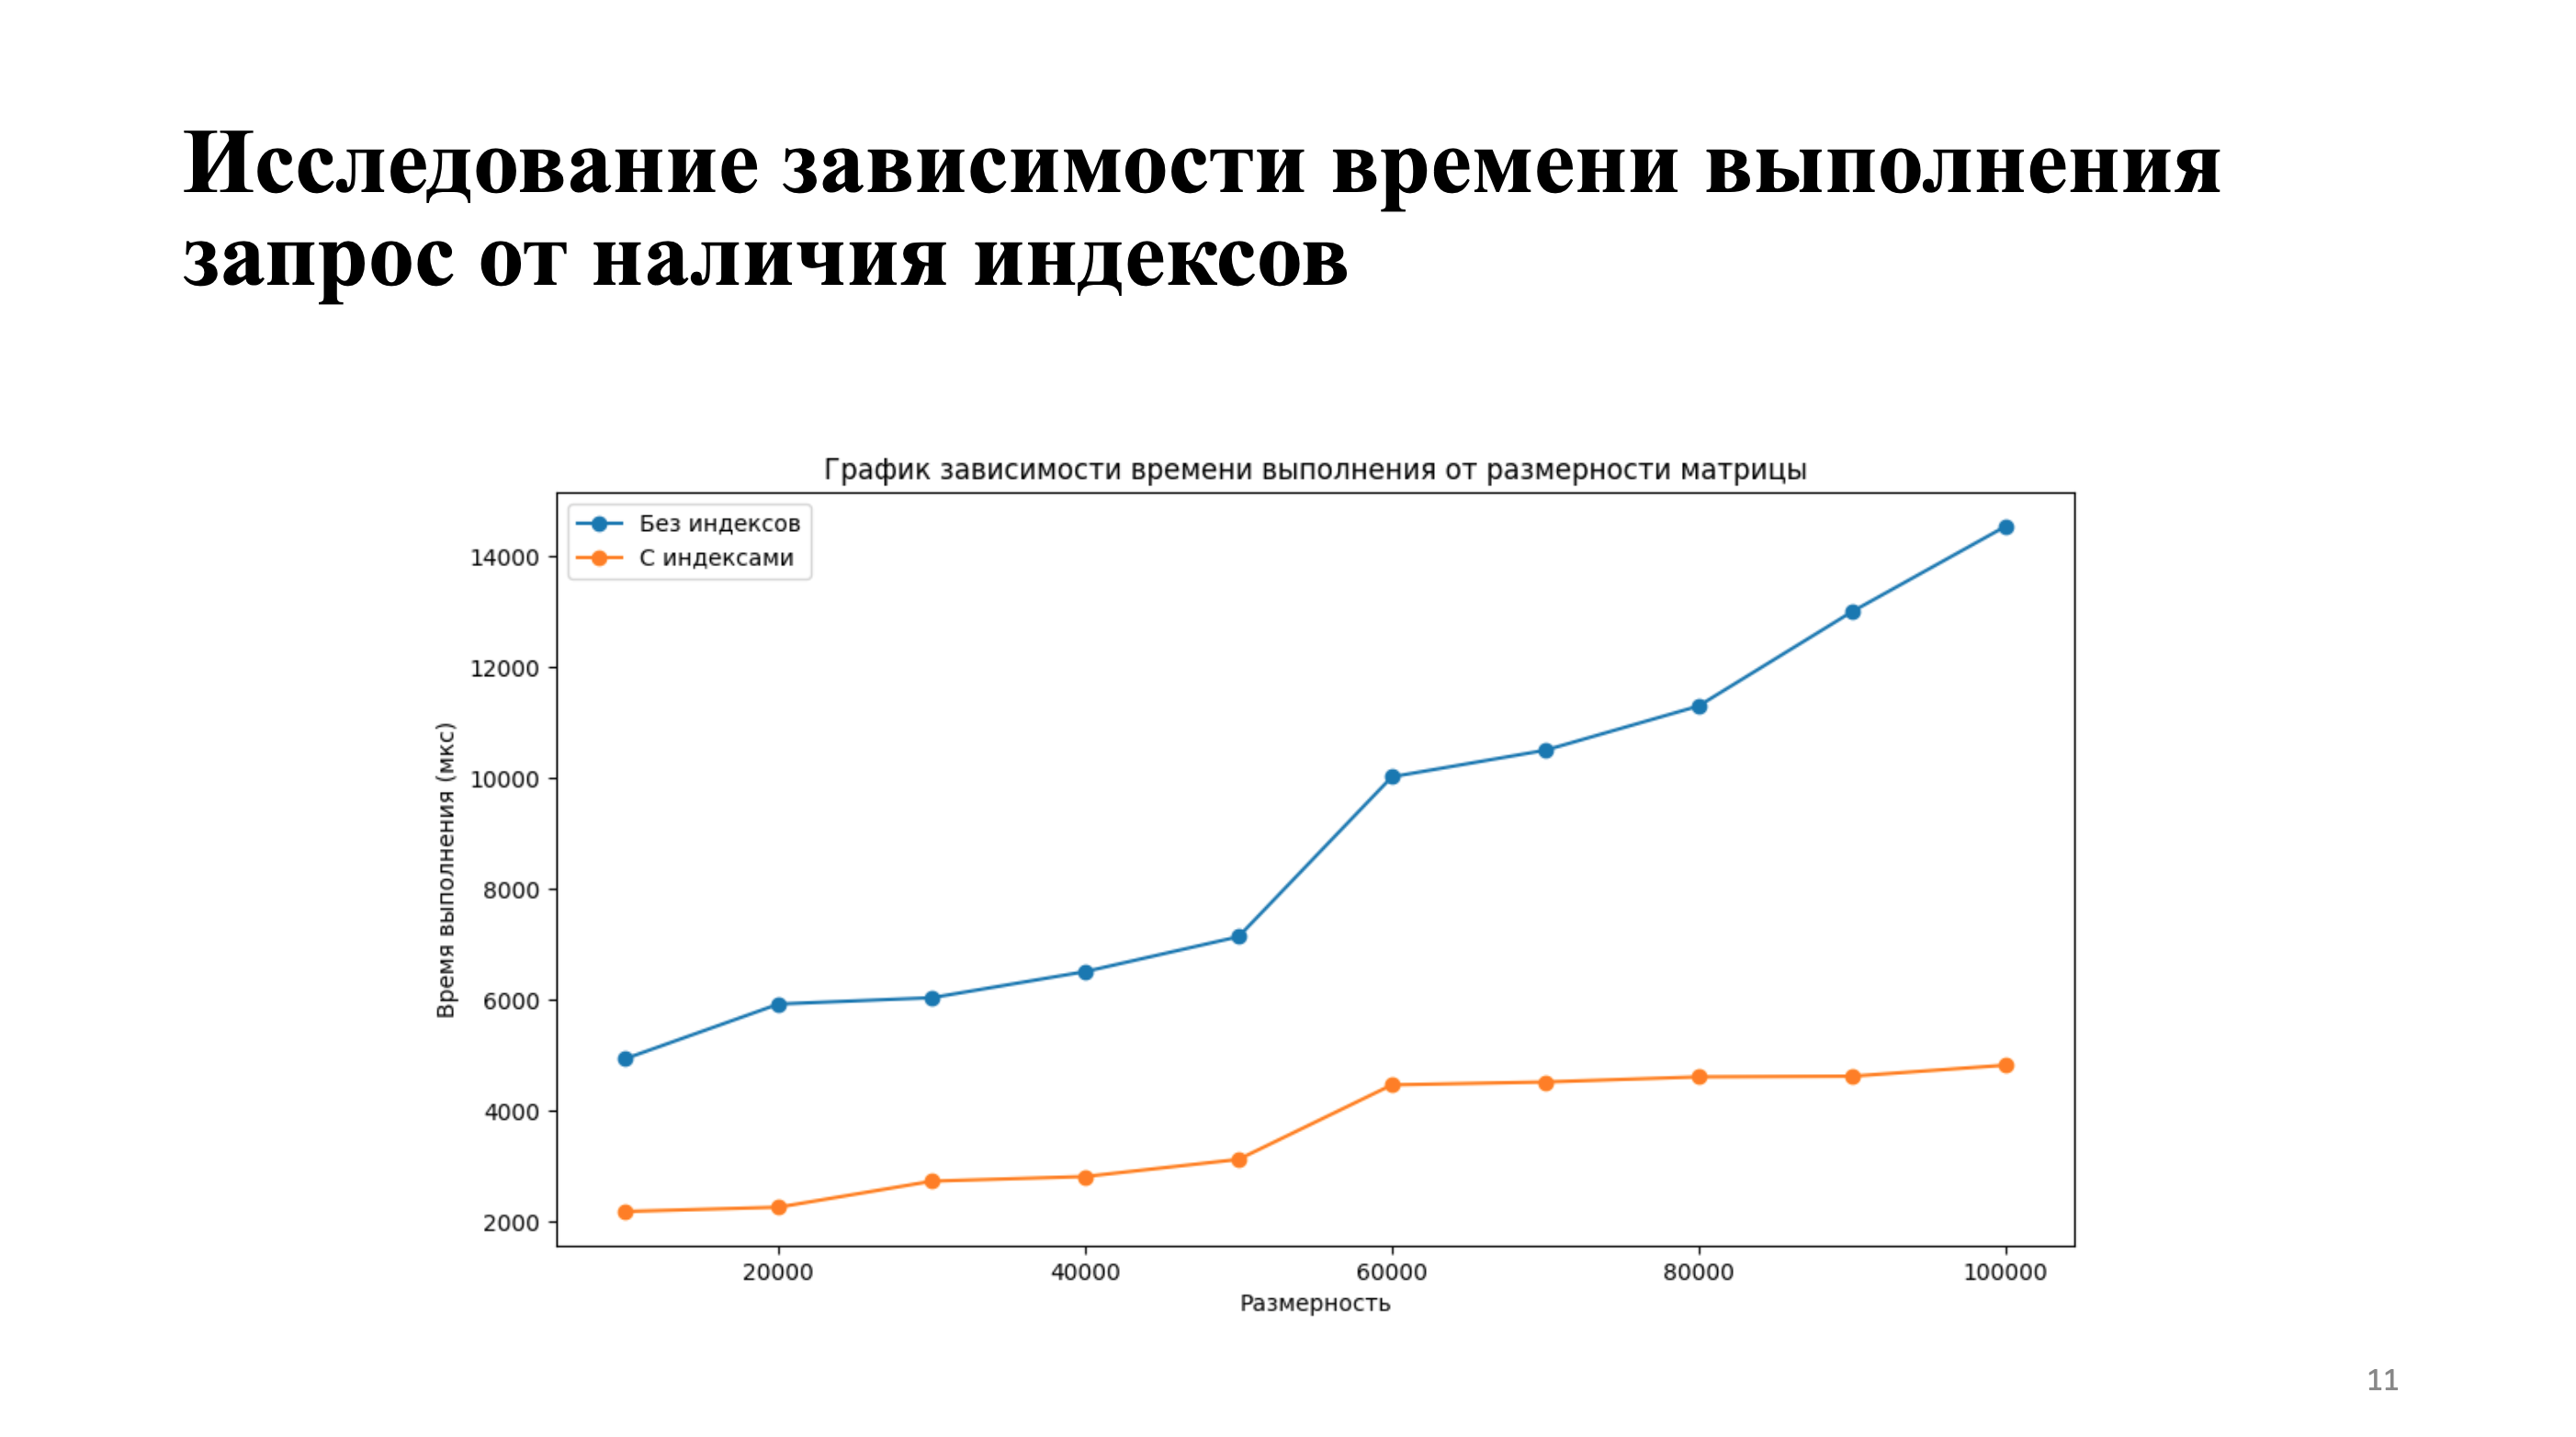
\includegraphics[width=1\linewidth]{img/11.png}
    \caption{Презентация -- слайд 11}
\end{figure}
\noindent

\begin{figure}[H]
    
\includegraphics[width=1\linewidth]{img/12.png}
    \caption{Презентация -- слайд 12}
\end{figure}
\noindent
